%\documentclass[14pt]{article}
\documentclass{article}
%\usepackage{extsizes}
\usepackage{amsfonts}
\usepackage{amsmath}
\usepackage[a4paper, inner=1.5cm, outer=2.5cm, top=2cm,
bottom=2cm, bindingoffset=1cm]{geometry}
\usepackage{graphicx}
\usepackage{subfigure}
\graphicspath{{img/}}  
\usepackage[section]{placeins}
\usepackage{afterpage}
\usepackage{titling}
\usepackage{siunitx}
\usepackage{epstopdf}
\usepackage{tikz}
\usepackage{bondgraph}
%\usepackage{cite}
\usepackage{booktabs}
\usepackage{caption}
\usepackage{color, colortbl}
\definecolor{Gray}{gray}{0.95}


\providecommand{\e}[1]{\ensuremath{\times 10^{#1}}}
\providecommand{\m}[1]{\ensuremath{\mathrm{#1}}}
\providecommand{\p}[1]{\ensuremath{\partial #1}}

\newcommand{\figWidth}{0.5\textwidth}
\newcommand{\subfigWidth}{0.45\textwidth}

\usepackage{todonotes}
\usetikzlibrary{shapes,arrows,decorations.markings}

\begin{document}
\title{Insulin-glucose interaction models}
\author{J\'achym Barv\'inek, Ji\v r\'i Figura, Martin Gurtner}

\maketitle

% ------------------------- Biological background  -------------------------
\section{Introduction}

The goal of this project is to get familiar with mathematical description of the nutrient utilization in the bloodstream of the human body. This problem can be studied as a simplified glucose-insulin interaction.
%The goal of this project is to get familiar with simplified mathematical description of the glucose-insulin interaction in the bloodstream of the human body. 
A short introduction to the underlying biological background is followed by a detailed mathematical derivation of V. Bolie's model~\cite{bolie1961coefficients} and its discussion.
Subsequently another, less general, model of insulin-glucose interaction by Bellomo et al. is briefly examined.
Before concluding with a review of the Ackerman's diabetes test, the Bolie's model with parameters identified for healthy human is elaborated. 

%This project report is concluded by a review  the Ackerman's diabetes test. 

\section{Biological background}

Glucose is the main energy source for body cells. It is obtained directly from food or as a result of metabolism of other carbohydrates. Glucose is needed by all cells in the body, but nerve cells are of critical importance and there needs
to be glucose available for them at every instant. In accordance with these needs, the glucose
metabolism evolved as follows:
After a period of not eating, a constant level of glucose in the bloodstream should be established,
some glucose is consumed by cells and this loss is balanced by glucose in the form of glycogen
released by liver. When some carbohydrates are ingested, they shall be metabolised into glucose
and as a result, its concentration in the bloodstream increases. In this situation, the pancreas
releases the hormone insulin, which sends a signal to cells (other than nerve cells) that they should
now absorb more glucose from the bloodstream. At the same time, liver reacts to increased level of 
glucose in the bloodstream by absorbing it and converting it to glycogen for storage. Liver also 
decomposes the insulin. There are other hormones and factors which play a role in the metabolism
of glucose. Adrenaline, for example increases the amount of glucose in the bloodstream available
to cells. The concentration of this hormone is, however, difficult to measure precisely.
In the following text we thus consider insulin as the only significant hormone.

If the concentration of insulin in bloodstream is too high, then cells absorb most of the glucose 
and as a result, there may not be enough for the nerve cells, which may end up by coma or death.
If the level of insulin is too low, then cells cannot obtain the energy they need for normal functioning.
The later is the case which happens for people suffering by the disorder Diabetes Mellitus -- their bodies
create insufficient amount of insulin.


% ------------------------- Bolie's diabetes model -------------------------
\section{Bolie's glucose-insulin interaction model}

Bolie's diabetes model is based on the following general assumptions, taken from~\cite{fulford_modelling_1997}:

\begin{enumerate}
	\item
	Insulin is being degraded by the liver.	
	\item
	A rise in the concentration of glucose in the bloodstream results in increased production of insulin by the pancreas.
	\item
	With increasing concentration of insulin, the glucose is more easily absorbed by the cells, i.e. it leaves the bloodstream more quickly.
	\item
	A rise in glucose concentration in the bloodstream results in increased glucose absorption by the liver.

\end{enumerate}


The model, described by eq.~\ref{eqbolie}, takes into account just two variables -- glucose $G$ and hormone insulin, denoted by $H$. Generally nonlinear functions on the right hand side of the equations follow directly from the assumptions above. The symbols with their corresponding meaning and units are summarized in Tab.~\ref{tabParam}. 

\begin{equation}
\label{eqbolie}
\begin{aligned}
V\frac{\m{d} H}{\m{d} t}&=-F_1(H)+F_2(G)+ x,\\
V\frac{\m{d} G}{\m{d} t}&=-F_3(H,G)-F_4(H,G) + y. 
\end{aligned}
\end{equation}

For changes around equilibrium $H_0$, $G_0$ we can rewrite the model to:

\begin{equation}
\label{eqbolieEquilibrium}
\begin{aligned}
V\frac{\m{d}h}{\m{d}t}&=-F_1(H_0+h)+F_2(G_0+g)+ x,\\
V\frac{\m{d}g}{\m{d}t}&=-F_3(H_0+h,G_0+g)-F_4(H_0+h,G_0+g)+ y.
\end{aligned}
\end{equation}

For small changes around the equilibrium it is possible to use linearized model. By Taylor expanding the eq.~\ref{eqbolieEquilibrium} with zero inputs we get:

\begin{align*}
\frac{\m{d}h}{\m{d}t}&=-\underbrace{%
		\frac{1}{V}\frac{\p F_1(H_0)}{\p H}}_{\alpha}h+%
%
\underbrace{%
		\frac{1}{V}\frac{\p F_2(G_0)}{\p G}}_{\beta}g+\mathcal{O}(2), \\%		
%
\frac{\m{d}g}{\m{d}t}&=-\frac{1}{V}\frac{\p F_3(H_0, G_0)}{\p H}h- \frac{1}{V}\frac{\p F_3(H_0, G_0)}{\p G}g-\frac{1}{V}\frac{\p F_4(H_0, G_0)}{\p H}h-\frac{1}{V}\frac{\p F_4(H_0, G_0)}{\p G}g+\mathcal{O}(2)\\%
%
&=-\underbrace{%
\frac{1}{V}\left(\frac{\p F_3(H_0, G_0)}{\p H}+\frac{\p F_4(H_0, G_0)}{\p H}\right)}_{\gamma}h%
-\underbrace{%
\frac{1}{V}\left(\frac{\p F_3(H_0, G_0)}{\p G}+\frac{\p F_4(H_0, G_0)}{\p G}\right)}_{\delta} g+\mathcal{O}(2).
\end{align*}

By omitting the second and higher order terms we get the following linear model:
\begin{equation}
\label{eqLinearized}
\begin{aligned}
\frac{\m{d}h}{\m{d}t}&=-\alpha h + \beta g,\\
\frac{\m{d}g}{\m{d}t}&=-\gamma h - \delta g.\\
\end{aligned}
\end{equation}

All of the constants $\alpha$, $\beta$, $\gamma$, $\delta$ are positive. Let's check that the signs correspond to Bolie's assumptions. If we put $g=0$ we can see from the first equation that the concentration of insulin decreases in time, which is in agreement with the first assumption.
On the other hand, if we put $h=0$ we can see that increase in $g$ leads to increase in $h$, which is in accordance with the second assumption.
Assumptions 3 and 4 say that rise in each of the variables results in   decrease of glucose concentration and the negative signs at both terms in the second equation reflect that.   

\begin{table}[h]
\renewcommand{\arraystretch}{1.1}  
\centering
\begin{tabular}{lll}
\toprule
\textbf{Symbol}  & \textbf{Meaning} & \textbf{Dimension}\\
\midrule
$V$ & volume & \si{\liter}\\
\rowcolor{Gray}
$x$ & rate of insulin injection & units \si{\per\hour}\\

$y$ & rate of glucose injection & \si{\gram\per\hour}\\
\rowcolor{Gray}
$H$ & insulin concentration & units \si{\per\liter}\\
$H_0$ & insulin concentration equilibrium & units \si{\per\liter}\\
\rowcolor{Gray}
$h$ & insulin concentration changes & units \si{\per\liter}\\
$G$ & glucose concentration & \si{\gram\per\liter}\\
\rowcolor{Gray}
$G_0$ & glucose concentration equilibrium & \si{\gram\per\liter}\\
$g$ & glucose concentration changes & \si{\gram\per\liter}\\
\rowcolor{Gray}
$F_1(H)$ & rate of insulin destruction & units \si{\per\hour}\\
$F_2(G)$ & rate of insulin production & units \si{\per\hour}\\

\rowcolor{Gray}
$F_3(H,G)$ & rate of liver accumulation of glucose & \si{\gram\per\hour}\\
$F_4(H,G)$ & rate of tissue utilization of glucose & \si{\gram\per\hour}\\
\bottomrule
\end{tabular}
\caption{Diabetes model parameters.}
\label{tabParam}
\end{table}

% ------------------------- Linearized model solution -------------------------
\section{Linearized model solution}

We can reduce the linearized model from eq.~\ref{eqLinearized} to a 2\textsuperscript{nd} order differential equation by differentiating the second equation and substituting $\dot h$ with the right hand side of the first equation:
%
\begin{equation*}
\ddot g=-\gamma \dot g -\delta \alpha g + \delta \beta h.
\end{equation*}
%
 The $h$ term is then substituted with the expression for $h$ derived from the second equation:
% 
\begin{equation}
\label{eq:hterm}
h = -\frac{1}{\gamma}\left( \dot{g} + \delta\,g\right).
\end{equation} 
%
We get:
\begin{equation}
	\label{Eq:secondOrderDE}
	\ddot g+(\gamma+\beta)\dot g+(\beta \gamma+\delta \alpha)g=0.
\end{equation}
%where $S(t)$ is a nonhomogeneous term reflecting external glucose input to the bloodstream.  
%
The solutions are found by solving the characteristic polynomial:
%
\begin{equation}
	\label{Eq:charEqn}
	\lambda^2+(\gamma+\beta)\lambda+(\beta\gamma+\delta\alpha)=0,
\end{equation}

\begin{equation}
	\label{Eq:rootsOfCharEqn}
	\lambda_{1,2}=\frac{1}{2}\left(-(\gamma+\beta)\pm \sqrt{(\gamma+\beta)^2-4(\beta\gamma+\delta\alpha)}\right).
\end{equation}
%
Since both $(\gamma+\beta)$ and $(\beta\gamma+\delta\alpha)$ are positive, the solutions are always stable, going to zero with $t\rightarrow \infty$. If the discriminant is lower than zero then the solutions go to zero periodically, otherwise aperiodically.\\
%
%
General solution is in the form:
\begin{equation}
	\label{Eq:genSol}
	g(t) = A\,e^{\lambda_1 \, t} + B\,e^{\lambda_2 \, t}.
\end{equation}
%
By specifying initial conditions $g(t_0=0) = g_0$ and $h(t_0=0)=0$ we can derive initial condition for $\dot g(t_0=0)$ by substituting $g_0$ for $g$ in eq.~\ref{eq:hterm}, thus obtaining $\dot g(t_0=0)=-\delta g_0$.\\
%
Constants A and B for the specified initial conditions are:
%
\begin{equation*}
	\label{Eq:genSolParams}
	A = g_0\,\frac{\delta+\lambda_2}{\lambda_2-\lambda_1}, \qquad B = g_0\,\frac{\delta+\lambda_1}{\lambda_1-\lambda_2}.
\end{equation*}

\section{Bellomo's model}
Bellomo et al. \cite{bellomo} suggest a more specific model of the glucose-insulin system, described by the following equations:
\begin{equation}
\label{Eq:bellomo}
\begin{aligned}
 \frac{\m{d}i}{\m{d}t} &= -\underbrace{K_{\mathrm{i}}\,i}_{F_1} + \underbrace{K_{\mathrm{g}}\,(g - g_{\mathrm{d}})}_{F_2} + \underbrace{K_{\mathrm{s}}\,i_{\mathrm{r}}}_{x}, \\
 \frac{\m{d}g}{\m{d}t} &= \underbrace{K_{\mathrm{h}}\,g - K_0\,g\,i - K_{\mathrm{s}}\,K_{\mathrm{f}}}_{-F_3-F_4} + \underbrace{0}_{y}.
\end{aligned}
\end{equation}
Where $i$ is the level of insulin and $g$ level of glucose.
Parameters $K_{\mathrm{i}}, K_{\mathrm{g}}, K_{\mathrm{s}}, K_{\mathrm{h}}, K_{\mathrm{f}}$ and also $g_{\mathrm{d}}$ are some constant coefficients.
Detailed description of their meaning can be found in \cite{bellomo}.
Finally $i_{\mathrm{r}}$ represents the rate of insulin infusion (or ingestion) and it's a function of $t$.
We use notation from the original paper, but Bellomo's model is a special case of the general Bolie's model.
In the underbraces, we can see the correspondence between parts of the equations \eqref{Eq:bellomo} to the Bolie's model \eqref{eqbolie}.

The meaning of the term $-K_{\mathrm{i}}\,i$ in the first equation is analogous to the term $-\alpha\,h$ in \eqref{eqLinearized},
furthermore the term $K_{\mathrm{g}}\,(g - g_{\mathrm{d}})$ has similar meaning as $\beta\,g$ in \eqref{eqLinearized},
except that it takes into account the reduction of insulin deliverance, which occurs during hypoglycemia 
(low level of blood sugar). This is done by substracting the constant $g_{\mathrm{d}}$.
An infusion of insulin of course increases it's level in bloodstream, so we add $i_r$ multiplied by a coefficient
to the change of insulin in time. The constant $K_{\mathrm{s}}\,K_{\mathrm{f}}$ represents some residual processes in the body,
which are not of big interest for us. The terms $K_{\mathrm{h}}\,g - K_0\,g\,i$, on the other hand,
are more significant. Their meaning can be probably better understood if we rewrite it like this:
\[ K_{\mathrm{h}}\,g - K_0\,g\,i = K_{\mathrm{n}}\,g\left(1 - \frac{K_0}{K_{\mathrm{n}}}\,i\right) := K_{\mathrm{n}}\,g(1 - a\,i). \]
Now we can see, that the the level of glucose in bloodstream can actually be growing, if
the value of $i$ is sufficiently small.
This is due to a certain time delay between glucose infusion and insulin release.
Otherwise, however, both glucose level and insulin levels affect the change of glucose negatively,
as in the case of equation \eqref{eqLinearized}.

%This system has two equilibrium points. Both of them can be shown to be unstable, assuming that $i_r(t) \ge 0$ for given $t$.
%The calculations leading to this result as well as the expressions of values of the equilibrium points themselves
%are very complicated and do not provide much insight to the problem, so we just state this as a fact.
% ^ Pravděpodobně bullshit, ale nechtěl jsem to mazat.

% ------------------------- Testing for diabetes -------------------------

\section{Testing for diabetes}
Now we will make use of the diabetes model. Probably the main purpose of developing such a model is to find a test which recognizes whether a patient has a diabetes or not. We will discuss two tests developed in early sixties, where each of them has a very similar criterion but uses the above derived model in slightly different way.
% -----  Bolie's test -------
\subsection{Bolie's test}
Bolie~\cite{bolie1961coefficients} identified all parameters of the model described by equations~\eqref{eqLinearized} for a healthy person via three methods. Two of them were based on measurements of changing glucose concentration of rabbits and dogs. The identified parameters were then extrapolated to humans. The third method utilized data from standard Glucose Tolerance Tests (GTT). He assumed that the response of glucose concentration is critically damped. Then he identified all parameters of the analytical response from measured data and recalculated them to parameters $\alpha$, $\beta$, $\gamma$ and $\delta$. The averaged parameters obtained by all three methods are summarized in Table~\ref{tabIdentParam}.

\begin{table}[!h]
\renewcommand{\arraystretch}{1.1}  
\centering
\begin{tabular}{lll}
\toprule
\textbf{Symbol}  & \textbf{Value} & \textbf{Dimension}\\
\midrule
$\alpha$ & $0.780$ & \si{\per\hour}\\
\rowcolor{Gray}
$\beta$ & $0.208$ & \si{unit\per\hour\per\gram}\\
$\gamma$ & $4.34$ & \si{\gram\per\hour\per unit}\\
\rowcolor{Gray}
$\delta$ & $2.92$ & \si{\per\hour}\\
\bottomrule
\end{tabular}
\caption{Identified parameters of Bolie's model}
\label{tabIdentParam}
\end{table}

By substitution of the identified parameters from Table~\ref{tabIdentParam} into equation~\eqref{Eq:rootsOfCharEqn} we get two distinct real roots
\begin{equation*}
	\lambda_1 = -1.36, \qquad 	\lambda_2 = -2.34.
\end{equation*}

Time response of glucose concentration can be easily obtained through substitution of the roots $\lambda_1$ and $\lambda_2$ into the equations~\eqref{Eq:genSolParams} and \eqref{Eq:genSol}.
\begin{equation}
	g(t) = g_0 \left( -0.59 e^{\lambda_1\,t} + 1.59 e^{\lambda_2\,t} \right)
\end{equation}

Now we can determine the time $t_\m{r}$ when the glucose concentration returns to its steady-state value. For this purpose we put $g(t)$ from equation~\eqref{Eq:genSol} equal to zero and then it directly follows
\begin{equation*}
	0 = A\,e^{\lambda_1 \, t_\m{r}} + B\,e^{\lambda_2 \, t_\m{r}}		\quad\Rightarrow\quad
	e^{\lambda_1\,t_\m{r}} = -\frac{B}{A}\,e^{\lambda_2\,t_\m{r}} 	\quad\Rightarrow\quad
	t_\m{r} = \frac{1}{\lambda_1 - \lambda_2}\,\m{ln}\left(-\frac{B}{A}\right).
\end{equation*}
%\begin{align*}
%	0 &= g_0 \left( -0.59 e^{\lambda_1\,t_\m{r}} + 1.59 e^{\lambda_2\,t_\m{r}} \right) \\
%&\downarrow\\
%	0.59 e^{\lambda_1\,t_\m{r}} &= 1.59 e^{\lambda_2\,t_\m{r}} 	\\
%&\downarrow\\
%	t_\m{r} &= \frac{1}{\lambda_1 - \lambda_2}\,\m{ln}\left(\frac{1.59}{0.59}\right)
%\end{align*}


This can be further simplified by substitution of $A$ and $B$ from~\eqref{Eq:genSolParams} to
\begin{equation}
	t_\m{r} = \frac{1}{\lambda_1 - \lambda_2}\,\m{ln}\left(\frac{\lambda_1+\delta}{\lambda_2+\delta}\right).
\end{equation}

After substitution of all parameters we get time $t_\m{r}=1.01\,\si{\hour}$. This value corresponds to time when the glucose concentration returns to its original value after a glucose ingestion (for a healthy individual). Therefore the time $t_\m{r}$ can serve as a threshold which indicates whether an individual has diabetes or not. The graph of $g(t)$ is displayed in Fig.~\ref{Fig:boliesTestGlucose}.

As we already know the general solution for $g(t)$, we can easily obtain the solution for $h(t)$ by rewriting of the first equation in~\eqref{eqLinearized} to
\begin{equation}
	h(t) = -\frac{1}{\gamma}\left( \dot{g}(t) + \delta\,g(t)\right).
\end{equation}

This gives us
\begin{equation}
	h(t) = -\frac{1}{\gamma}\left[   A(\lambda_1 + \delta)e^{\lambda_1\,t} + B(\lambda_2 + \delta)e^{\lambda_2\,t}  \right] = K\,g_0 \left(e^{\lambda_1\,t} - e^{\lambda_2\,t} \right),
\end{equation}
where $$K=\frac{(\lambda_1+\delta)(\lambda_2+\delta)}{\gamma\,(\lambda_2-\lambda_1)}.$$

Now we can determine the time when the insulin concentration reaches its maximum. We simply find a local maximum of $h(t)$ by solving equation $\dot{h}(t_\m{m})=0$ in very similar way as we did it for the glucose concentration.
\begin{equation*}
	\dot{h}(t_\m{m}) = K\,g_0 \left( \lambda_1\,e^{\lambda_1 \, t} - \lambda_2\,e^{\lambda_2 \, t} \right) = 0		\quad\Rightarrow\quad
	e^{\lambda_1\,t_\m{m}} = \frac{\lambda_2}{\lambda_1}\,e^{\lambda_2\,t_\m{m}} 	\quad\Rightarrow\quad
	t_\m{m} = \frac{1}{\lambda_1 - \lambda_2}\,\m{ln}\left(\frac{\lambda_2}{\lambda_1}\right).
\end{equation*}

The time $t_\m{m}$ for the above identified parameters is $0.55\,\si{\hour}$. The function h(t) is depicted in Fig.~\ref{Fig:boliesTestInsulin}.

\begin{figure}[h!t!]
	\begin{center}
	\subfigure[Glucose concentration]{
		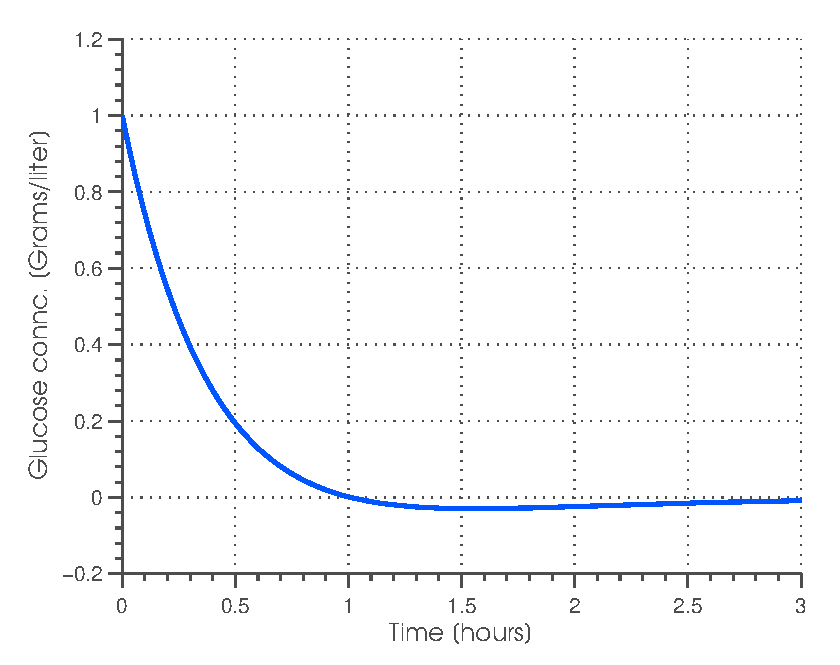
\includegraphics[width=\subfigWidth]{figs/boliesTestGlucose}
		\label{Fig:boliesTestGlucose}
	}
	\,
	\subfigure[Insulin concentration]{
		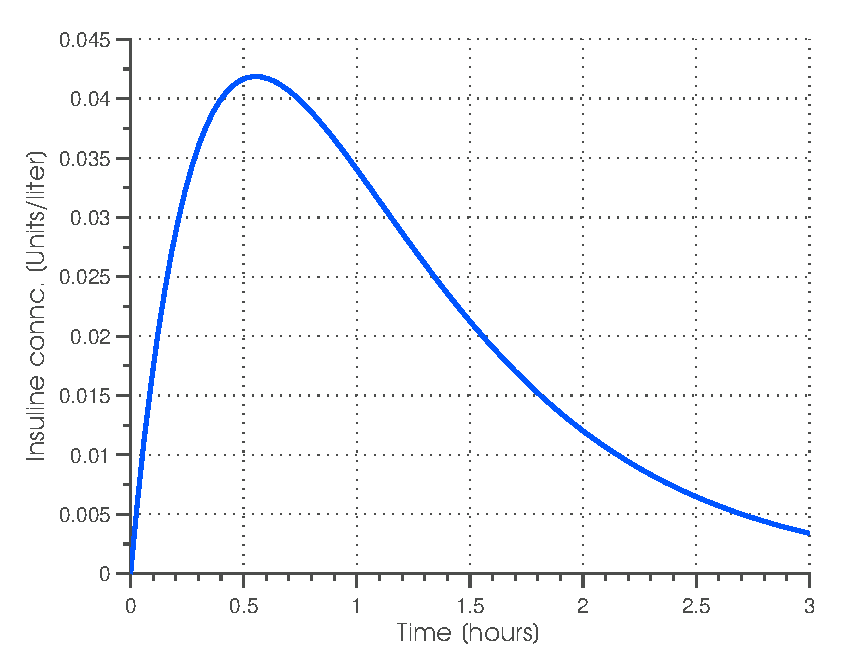
\includegraphics[width=\subfigWidth]{figs/boliesTestInsulin}	     
		\label{Fig:boliesTestInsulin}
	}
	\end{center}
	\caption{Time responses of glucose and insulin concentration after glucose ingestion ($g_0 = \SI{1}{\gram\per\liter}$)}
\end{figure}

% -----  Ackerman's diabetes test -------
\subsection{Ackerman's diabetes test}
An alternative approach to test diabetes is so called Ackerman's test~\cite{braun_differential_1983}. The test uses the same linearized model of blood glucose regulatory system as we described earlier in this report by system of equations~\eqref{eqLinearized}. If we neglect all inputs and reduce the system to one equation, we can also describe the same model by equation
\begin{equation}
	\label{Eq:AckerSecondOrder}
	\ddot g+2\sigma\,\dot g+\omega_0^2\,g=0,
\end{equation}
where $\nu$ and $\omega_0^2$ by simple comparison with~\eqref{Eq:secondOrderDE} are $\nu = (\alpha+\delta)/2$ and $\omega_0^2 = \beta\gamma+\alpha\delta$.

The solution of differential equation~\eqref{Eq:AckerSecondOrder} can be under-damped, over-damped and critically-damped depending on the value of the roots of the characteristic equation~\eqref{Eq:charEqn}. Ackerman assumed that the solution is always oscillatory (under-damped) and hence is of the form
\begin{equation}
%	g(t) = e^{-\sigma\,t}\left(  C_1\cos \omega t + C_2\sin \omega t    \right),
	g(t) = C\,e^{-\sigma t}\cos ( \omega t  - \varphi),
\end{equation}
where $\omega = \sqrt{\omega_0^2- \sigma^2}$. Finally, if we add the equilibrium value of the glucose concentration $G_0$, we get a function $G(t)$ in time which describes the overall glucose concentration in the blood system:
\begin{equation}
	\label{Eq:GT}
	G(t) = G_0 + C\,e^{-\sigma t}\cos ( \omega t  - \varphi)
\end{equation}

Function $G(t)$ has five parameters to identify. Two of them has quite straightforward interpretation which now will be given. Parameter $\sigma$ directly determines the time after which the system will be back in its equilibrium after some perturbations. Parameter $\omega$ describes the frequency of the oscillations in the response. One could expect that parameter $\alpha$ is better for classification if someone has diabetes or not. Nevertheless, it appears that it is difficult to identify $\alpha$ correctly, whereas $\omega_0$ doesn't suffer from this problem. Parameter $\omega_0$ can be further recalculated to the corresponding natural period $T_0=2\pi/\omega_0$. Ackerman observed that people, whose time response of the glucose concentration has smaller time 
$T_0$ than 4 hours, are healthy.

\paragraph{Example}
Table~\ref{tabAckerData} contains data from measurements of the glucose concentration collected during standard Glucose Tolerance Test for two persons~\cite{mahaffy}. The data for each of them were fitted with the function $G(t)$ from equation~\eqref{Eq:GT} by Leas Squares Method in Matlab. The identified parameters are summarized in Table~\ref{tabAckerParams} and the identified curves are depicted in Figure~\ref{Fig:ackerResult}. From the natural periods in Table~\ref{tabAckerParams} one can clearly see that the first person is healthy and the other one suffers from diabetes.

\begin{figure}[!h]
	\begin{minipage}[b]{0.48\textwidth}
		\centering
\renewcommand{\arraystretch}{1.1}  
\centering
\begin{tabular}{lll}
\toprule
\textbf{Time}  & \textbf{Data 1} & \textbf{Data 2}\\
\m{[hour]} & \m{[mg/dl]} & \m{[mg/dl]}\\
\midrule
0       &75      &100 \\
\rowcolor{Gray}
0.5     &160     &185 \\
0.75    &180     &210 \\
\rowcolor{Gray}
1       &155     &220 \\
1.5     &95      &195 \\
\rowcolor{Gray}
2       &75      &175 \\
2.5     &65      &105 \\
\rowcolor{Gray}
3       &80      &100 \\
4       &85      &85 \\
\rowcolor{Gray}
5       &80      &90 \\
\bottomrule
\end{tabular}
\captionof{table}{Data collected in standard GTT for two persons.\\}
\label{tabAckerData}
	\end{minipage}
	\hspace{0.04\textwidth}
	\begin{minipage}[b]{0.48\textwidth}
		\centering
\renewcommand{\arraystretch}{1.1}  
\centering
\begin{tabular}{lll}
\toprule
\textbf{Parameter}  & \textbf{Data 1} & \textbf{Data 2}\\
\midrule
$A$       			&175.8      	&222.7 \\
\rowcolor{Gray}
$G_0$     			&83.9    	&102.9 \\
$\alpha$   			&0.913     	&0.5582 \\
\rowcolor{Gray}	
$\omega$       		&1.87     	&1.12 \\
$\varphi$     			&1.633     	&1.591 \\
\rowcolor{Gray}
$\omega_0$       		&2.086      	&1.251 \\
$T_0$     			&3.019     	&5.023 \\
\bottomrule
\end{tabular}
%\vspace{31pt}
\captionof{table}{Identified parameters of the time responses of the glucose concentration from the example.}
\label{tabAckerParams}
	\end{minipage}
\end{figure}

\begin{figure}[h!t!]
   \centering
   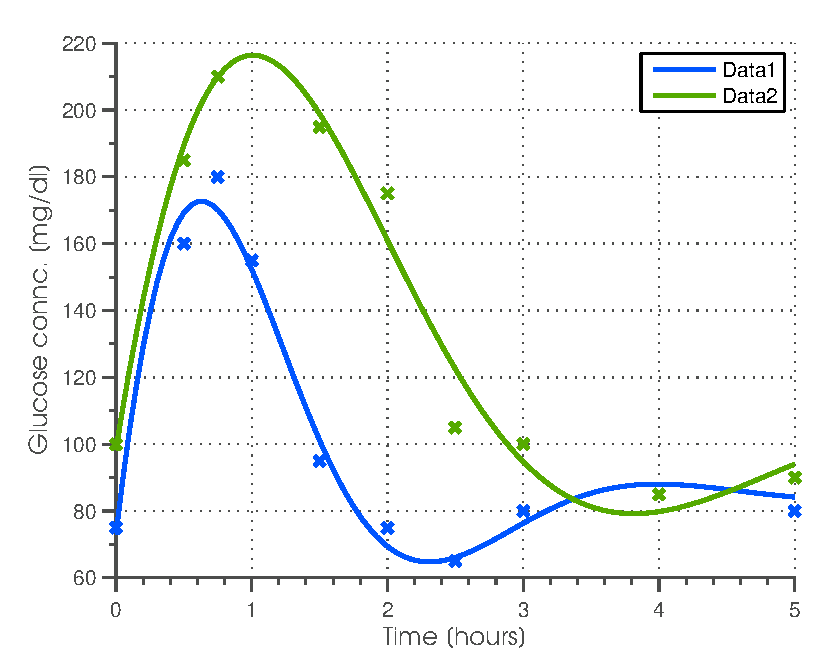
\includegraphics[width=\figWidth]{figs/ackermanTest1}
	\vspace{-5pt}
   \caption{Comparison of the measured glucose concentration with the identified model response.}
   \label{Fig:ackerResult}
\end{figure}

\bibliographystyle{IEEEtran}
\bibliography{DiabetesBibliography}

\end{document}
